\documentclass{../cssheet}

%--------------------------------------------------------------------------------------------------------------
% Basic meta data
%--------------------------------------------------------------------------------------------------------------

\title{Kongruenz -- Präsenzaufgaben}
\author{Prof. Dr. Christian Spannagel}
\date{\today}
\hypersetup{%
    pdfauthor={\theauthor},%
    pdftitle={\thetitle},%
    pdfsubject={Aufgabenblatt Inside Math!},%
    pdfkeywords={insidemath,aehnlichkeit,geometrie}
}

%--------------------------------------------------------------------------------------------------------------
% document
%--------------------------------------------------------------------------------------------------------------

\begin{document}
\printtitle

\vspace*{5mm}

\textbf{Aufgabe 1 (Symmetrie):}  Eine Symmetrieabbildung einer Figur ist eine Kongruenzabbildung, welche die Figur auf sich selbst abbildet. Wenn es sich um eine Achsenspiegelung handelt, dann ist die Figur achsensymmetrisch, bei einer Drehung drehsymmetrisch und bei einer Punktspiegelung punktsymmetrisch.
\begin{enumerate}[a)]
\item Welche Symmetrien haben folgende Figuren, und wie viele jeweils?
\begin{center}
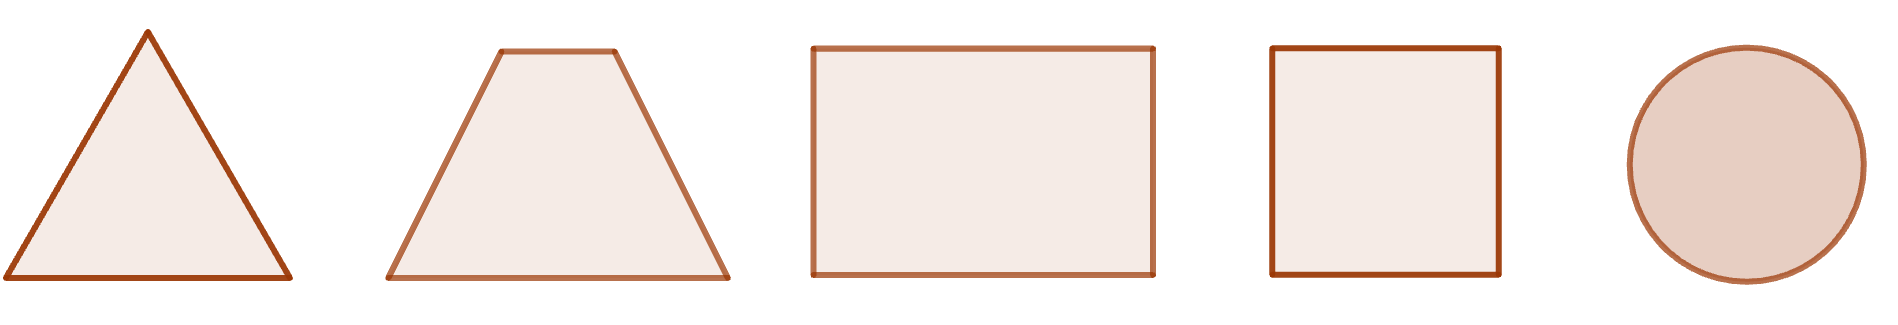
\includegraphics[width=10cm]{symmetrische-figuren.png}
\end{center} 
\item Zeichnet Figuren, die 1. gar keine Symmetrie haben, 2. Drehsymmetrien, aber keine Achsensymmetrie haben und 3. mindestens zwei Achsensymmetrien, aber keine Drehsymmetrien haben. (Hinweis: Bei dieser Aufgabe wird die Drehung um $0^\circ$ nicht betrachtet!)
\end{enumerate}


\textbf{Aufgabe 2 (Bandornamente):}  Bei Aufgabe~1 hatten wir Verschiebungen ausgenommen. Sobald wir eine Verschiebung zulassen, sind wir im Bereich der Bandornamente. In Bandornamenten können folgende Kongruenzabbildungen gefunden werden: Verschiebung, Längsspiegelung, Querspiegelung, Schubspiegelung und Drehung/Punktsymmetrie. Je nachdem, welche Kongruenzabbildungen vorhanden sind, kann man 7~Typen von Bandornamenten unterscheiden.

\begin{center}
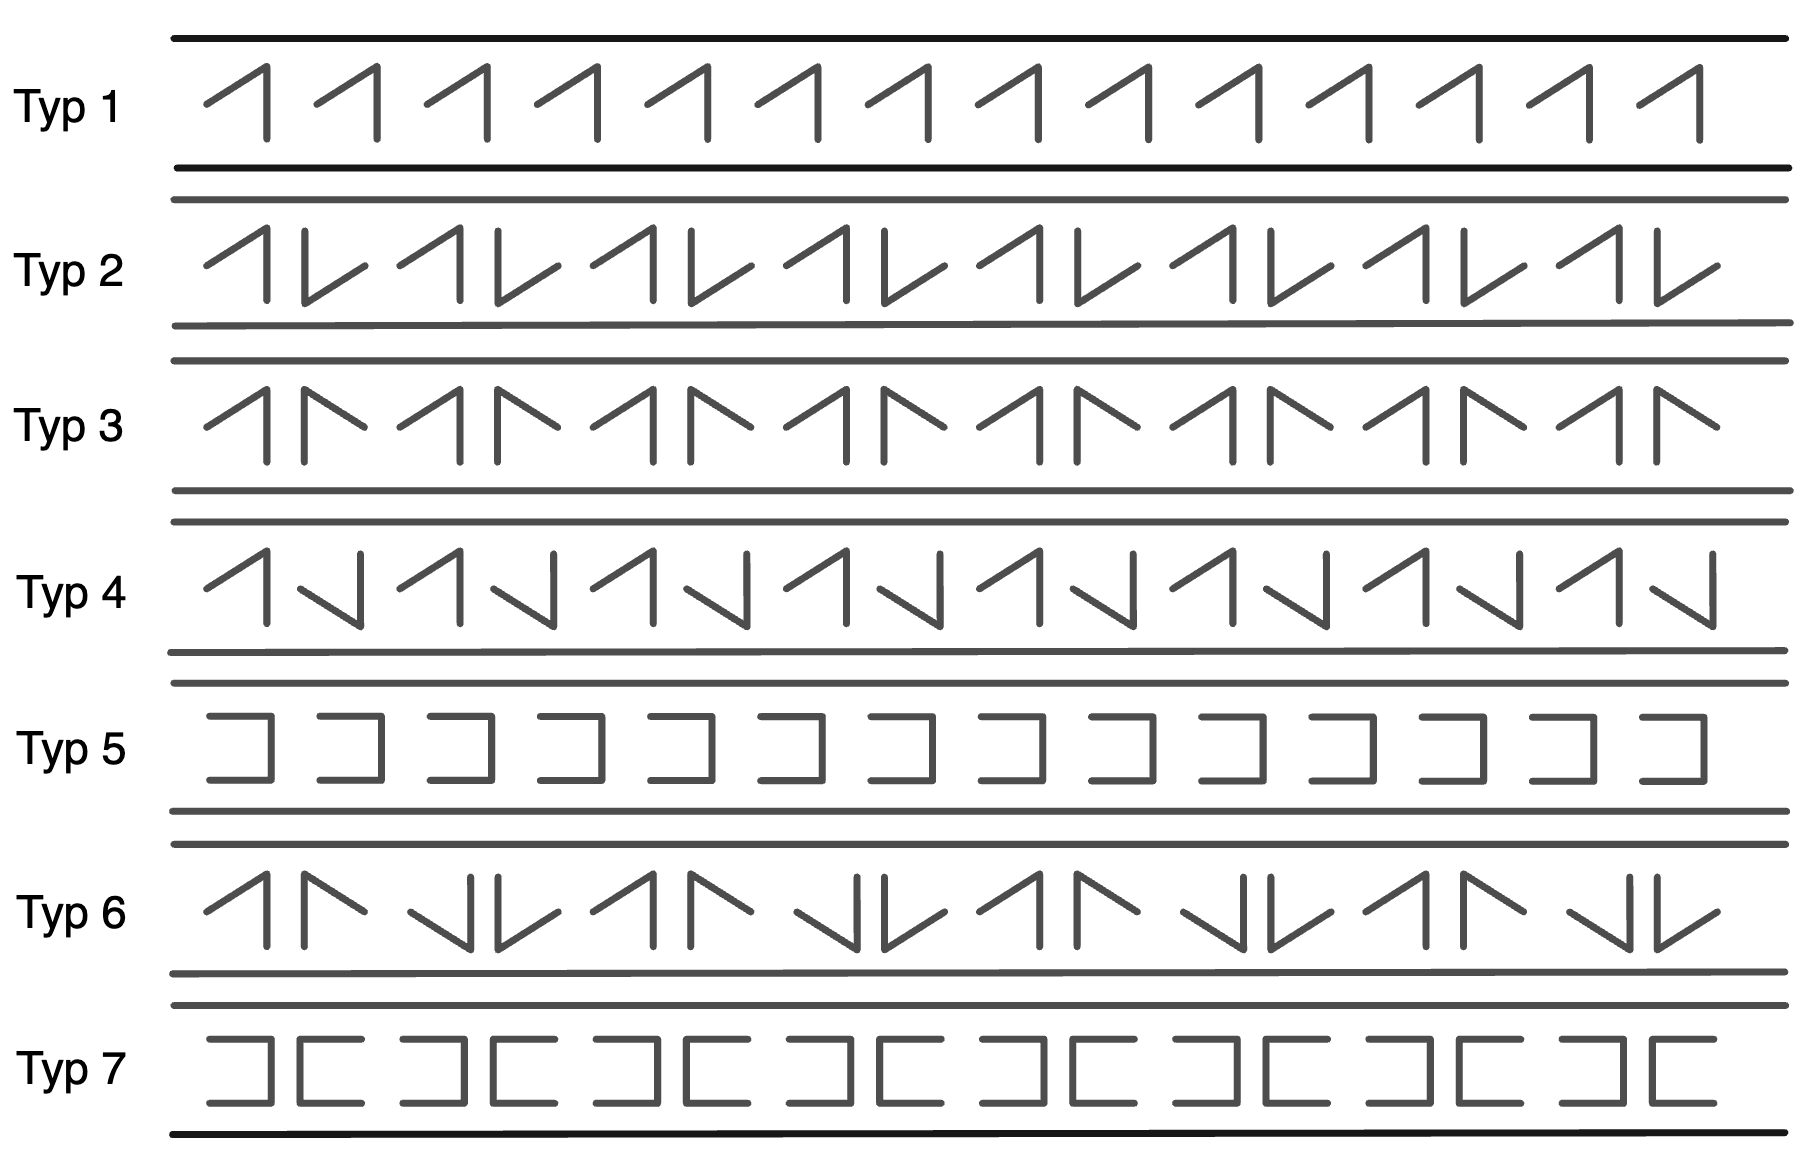
\includegraphics[width=10cm]{bandornamente.png}
\end{center} 

Schreibt für jeden der 7~Typen auf, welche Kongruenzabbildungen darin jeweils auftreten. Achtung: Ggf. müsst ihr unterschiedliche Grundfiguren betrachten.

Die Grafik zu Aufgabe~2 ist entlehnt an: Helmerich, M. \& Lengnink, K.. (2016). \emph{Einführung Mathematik Primarstufe -- Geometrie} (2.~Aufl.). Berlin, Heidelberg: Springer. S.~106

\newpage
\printlicense

\printsocials


\end{document}
